\documentclass[xcolor={dvipsnames},10pt]{beamer}

\usepackage{../style.sty/mybeamer}

\title[Industriedynamik]{Übung Industriedynamik}
\author{Dominic Görz, Daniel Horstmann}
\date{\today}
\setbeamertemplate{navigation symbols}{}%remove navigation symbols

\begin{document}

\begin{frame}
  \maketitle
\end{frame}

\begin{frame}{Contents}
  \tableofcontents
\end{frame}

\section{Fixe Strategien}

\subsection{Gewinne}

\begin{frame}{Gewinne (a)}
\begin{columns}[T]
    \begin{column}{.3\textwidth}
      \begin{itemize}
      \item Der Gewinn einer Firma steigt
      \item Die Gewinne der anderen Firmen fallen und erreichen den Wert Null
      \end{itemize}
      \end{column}
      \begin{column}{.7\textwidth}
      \begin{figure}[t]
            \centering
            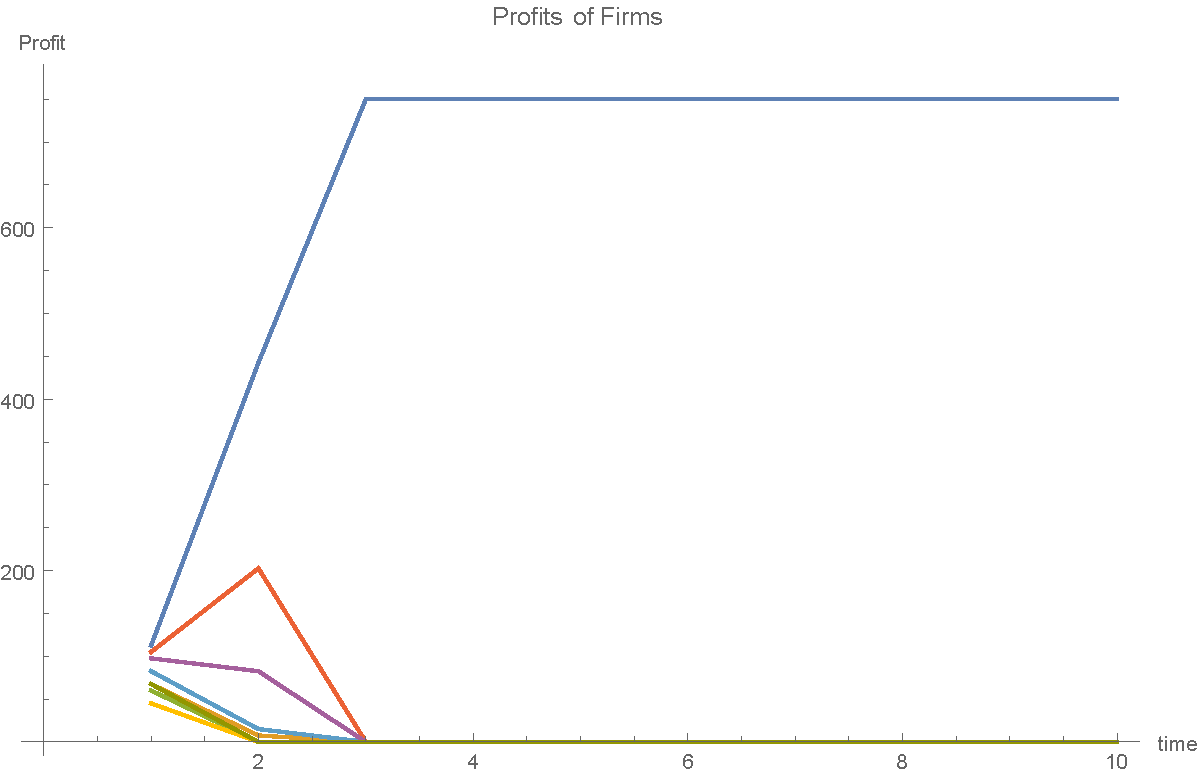
\includegraphics[scale=0.35]{../Plots/profit1a}
            \caption{Profite in 1 a)}
            \label{fig:profit1a}
       \end{figure}
    \end{column}
  \end{columns}
\end{frame}

\begin{frame}{Gewinne (b)}
\begin{columns}[T]
    \begin{column}{.3\textwidth}
      \begin{itemize}
      \item Die Gewinne der Firmen, welche die smarte Komponente einkaufen,
            scheinen um einen Mittelwert zu fluktuieren.
      \item Die Gewinne der Firmen, welche die smarte Komponente selber herstellen,
            sinken und erreichen den Wert Null
      \end{itemize}
      \end{column}
      \begin{column}{.7\textwidth}
      \begin{figure}[t]
            \centering
            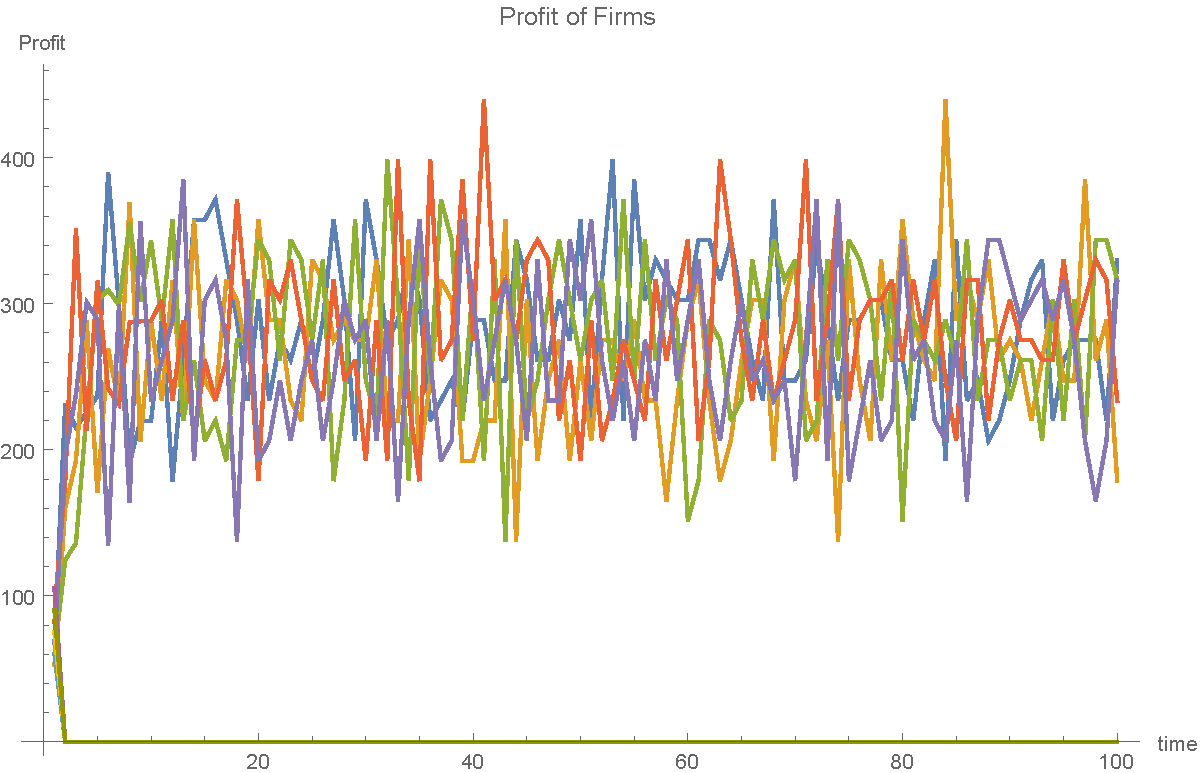
\includegraphics[scale=0.35]{../Plots/profit1b}
            \caption{Profite in 1 b)}
            \label{fig:profit1b}
       \end{figure}
    \end{column}
  \end{columns}
\end{frame}

\begin{frame}{Gewinne (c)}
\begin{columns}[T]
    \begin{column}{.3\textwidth}
      \begin{itemize}
      \item Die Gewinne aller Firmen scheinen um einen Mittelwert zu fluktuieren.
      \end{itemize}
      \end{column}
      \begin{column}{.7\textwidth}
      \begin{figure}[t]
            \centering
            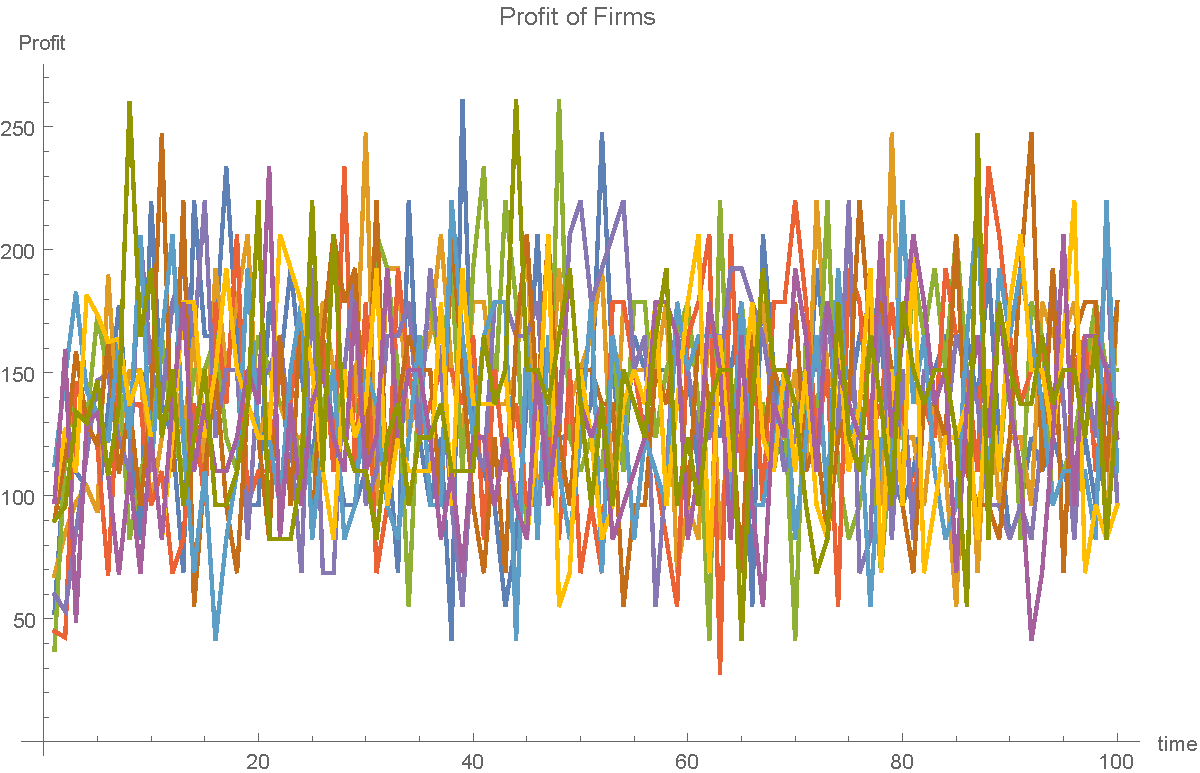
\includegraphics[scale=0.35]{../Plots/profit1c}
            \caption{Profite in 1 c)}
            \label{fig:profit1c}
       \end{figure}
    \end{column}
  \end{columns}
\end{frame}


\subsection{Qualität}

\begin{frame}{Qualität (a)}
\begin{columns}[T]
    \begin{column}{.3\textwidth}
      \begin{itemize}
      \item Qualität von Produkten der Firma, die sich durchsetzt, steigt
      \item Qualität von Produkten der anderen Firmen stagniert. 
      \end{itemize}
      \end{column}
      \begin{column}{.7\textwidth}
      \begin{figure}[t]
            \centering
            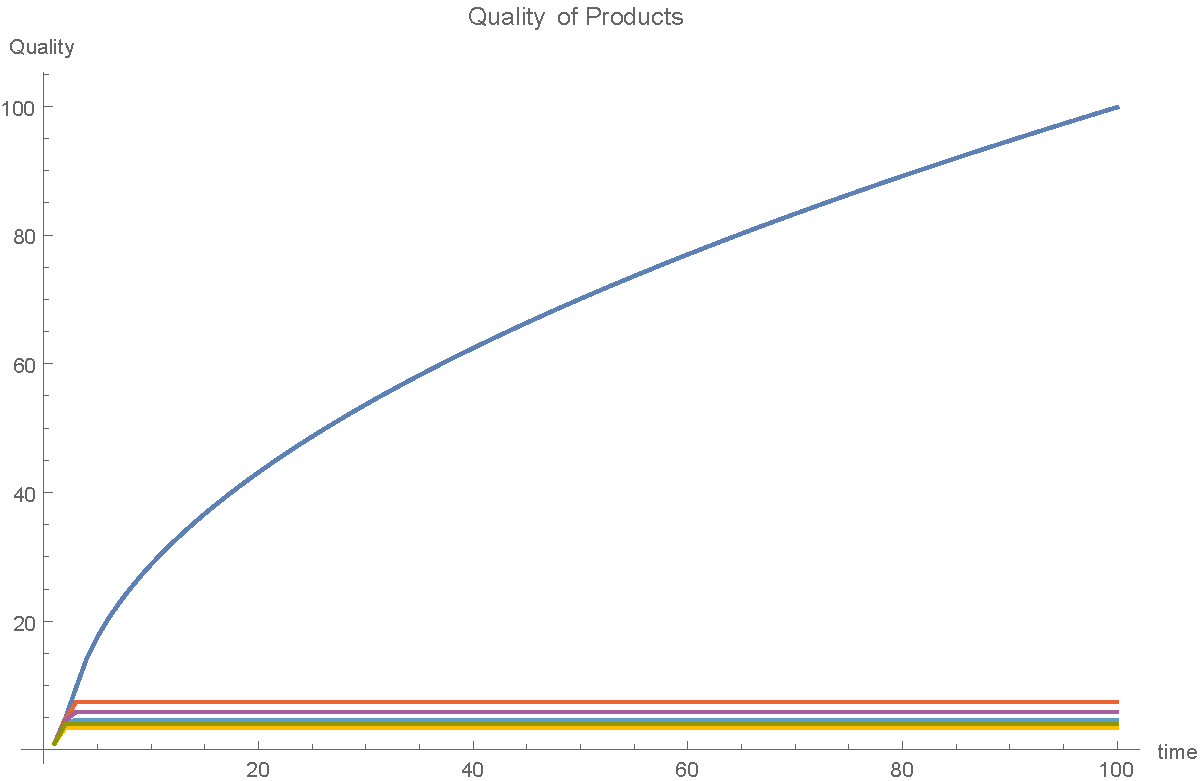
\includegraphics[scale=0.35]{../Plots/quality1a}
            \caption{Qualität in 1 a)}
            \label{fig:quality1a}
       \end{figure}
    \end{column}
  \end{columns}
\end{frame}

\begin{frame}{Qualität (b)}
\begin{columns}[T]
    \begin{column}{.3\textwidth}
      \begin{itemize}
      \item Qualität von Produkten der Firmen, welche die smarte Komponente einkaufen, ist identisch...
      \item ...und steigt
      \item Qualität von Produkten der anderen Firmen stagniert erneut 
      \end{itemize}
      \end{column}
      \begin{column}{.7\textwidth}
      \begin{figure}[t]
            \centering
            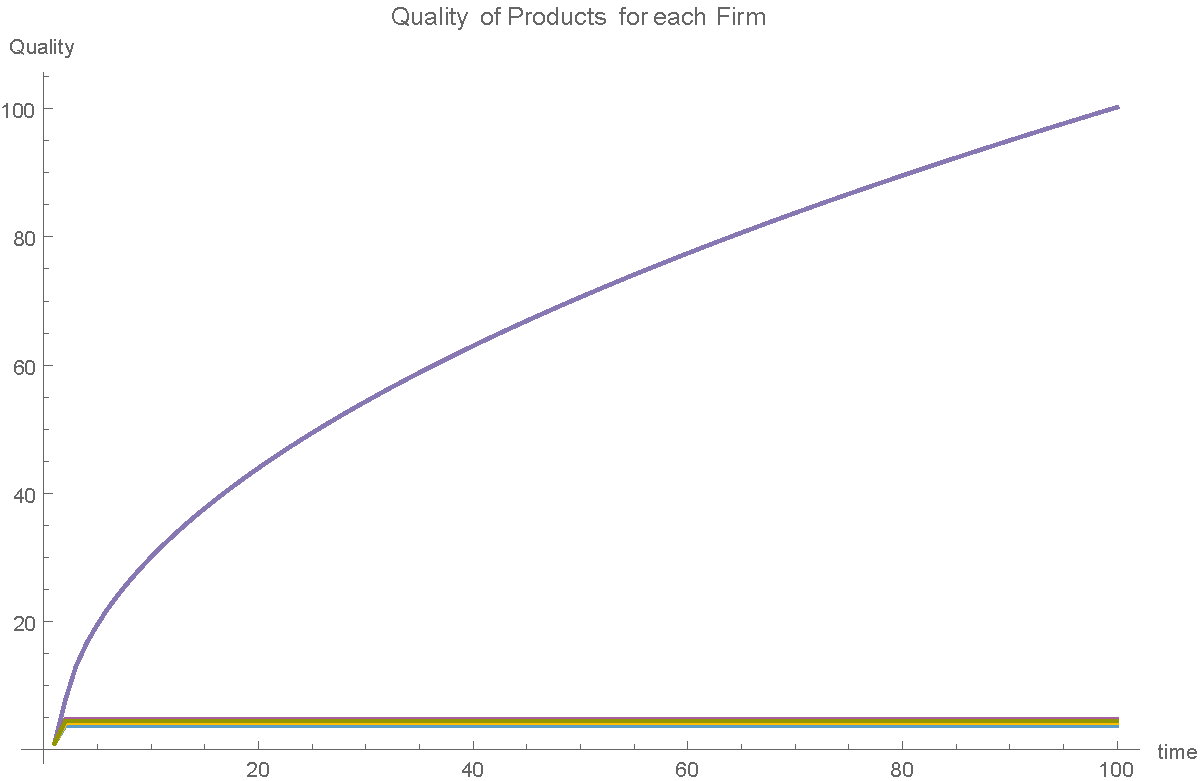
\includegraphics[scale=0.35]{../Plots/quality1b}
            \caption{Qualität in 1 b)}
            \label{fig:quality1b}
       \end{figure}
    \end{column}
  \end{columns}
\end{frame}

\begin{frame}{Qualität (c)}
\begin{columns}[T]
    \begin{column}{.3\textwidth}
      \begin{itemize}
      \item Qualität von Produkten aller Firmen ist identisch...
      \item ...weil die Qualität der Produkte nur von der Qualität der smarten Komponente abhängt
      \end{itemize}
      \end{column}
      \begin{column}{.7\textwidth}
      \begin{figure}[t]
            \centering
            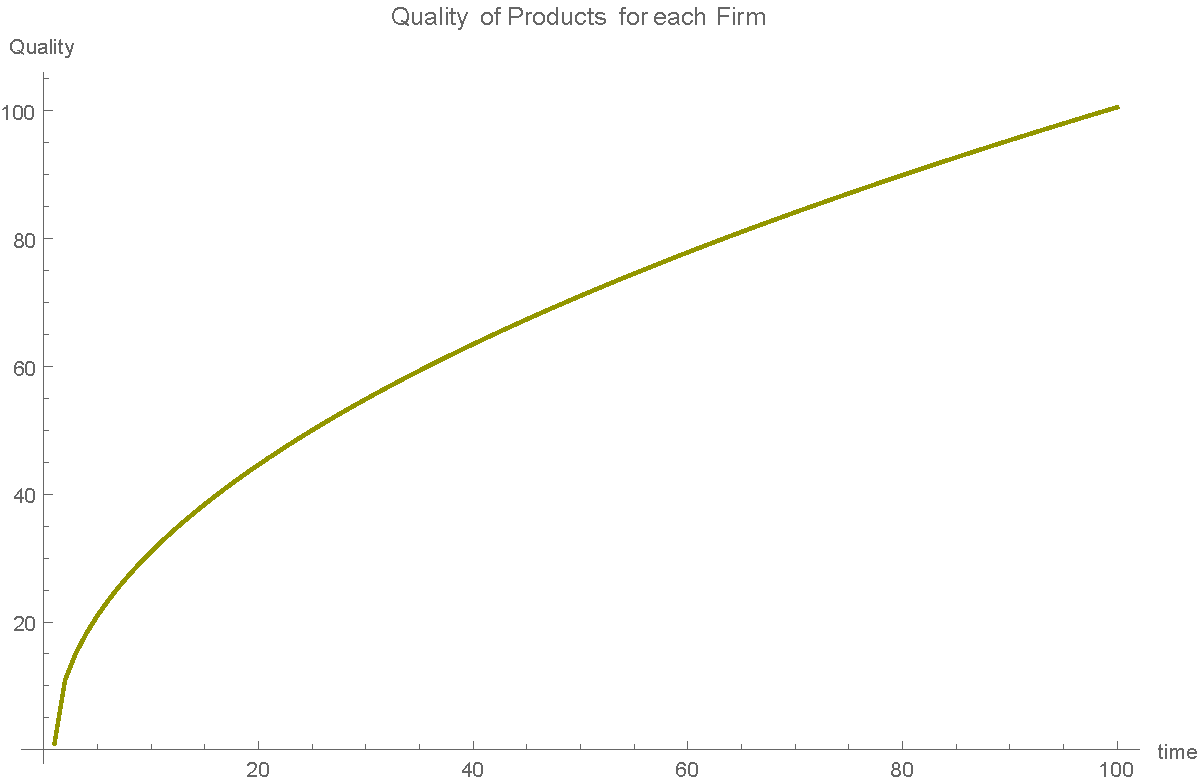
\includegraphics[scale=0.35]{../Plots/quality1c}
            \caption{Qualität in 1 c)}
            \label{fig:quality1c}
       \end{figure}
    \end{column}
  \end{columns}
\end{frame}

\subsection{Preise}

\begin{frame}{Preise (a)}
\begin{columns}[T]
    \begin{column}{.3\textwidth}
      \begin{itemize}
      \item Alle Preise sind identisch und konstant!
      \end{itemize}
      \end{column}
      \begin{column}{.7\textwidth}
      \begin{figure}[t]
            \centering
            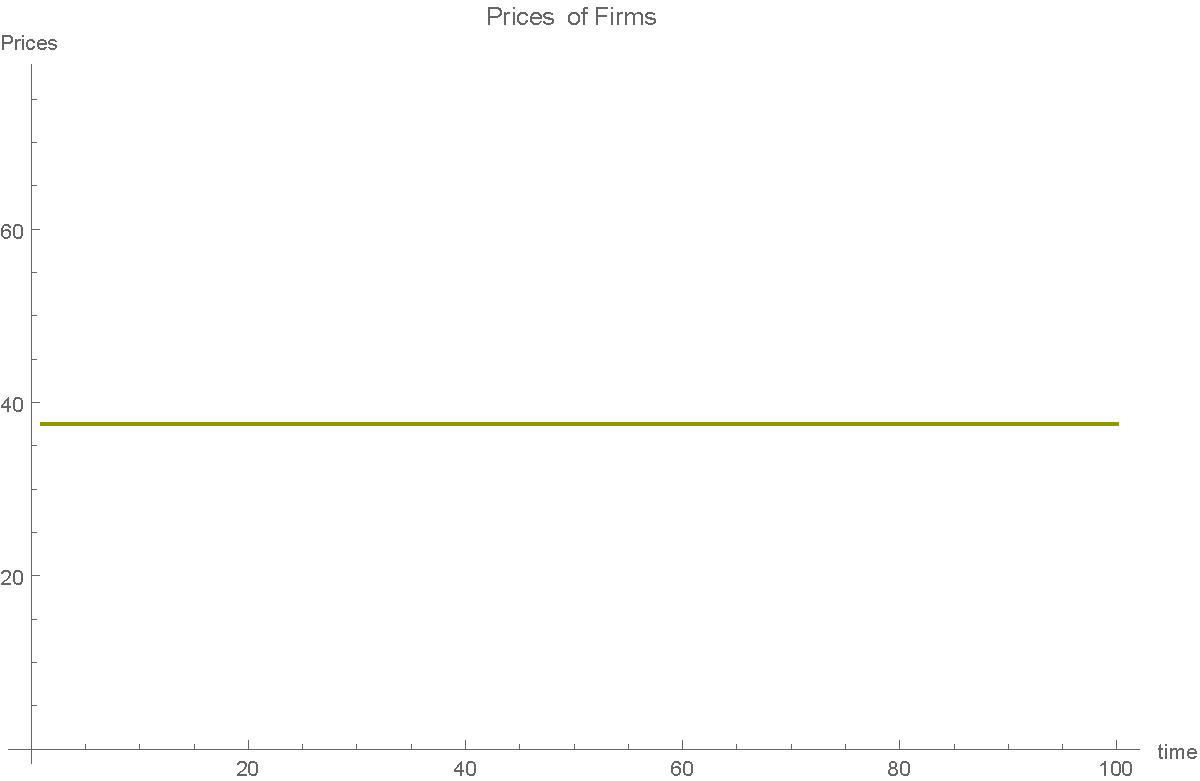
\includegraphics[scale=0.35]{../Plots/prices1a}
            \caption{Preise in a)}
            \label{fig:prices1a}
       \end{figure}
    \end{column}
  \end{columns}
\end{frame}

\begin{frame}{Preise (b)}
\begin{columns}[T]
    \begin{column}{.3\textwidth}
      \begin{itemize}
      \item Die Preise der Firmen, welche die smarte Komponente selber herstellen, sind identisch und konstant!
      \item Die Preise der Firmen, welche die smarte Komponente einkaufen, sind identisch und konvergieren.
      \end{itemize}
      \end{column}
      \begin{column}{.7\textwidth}
      \begin{figure}[t]
            \centering
            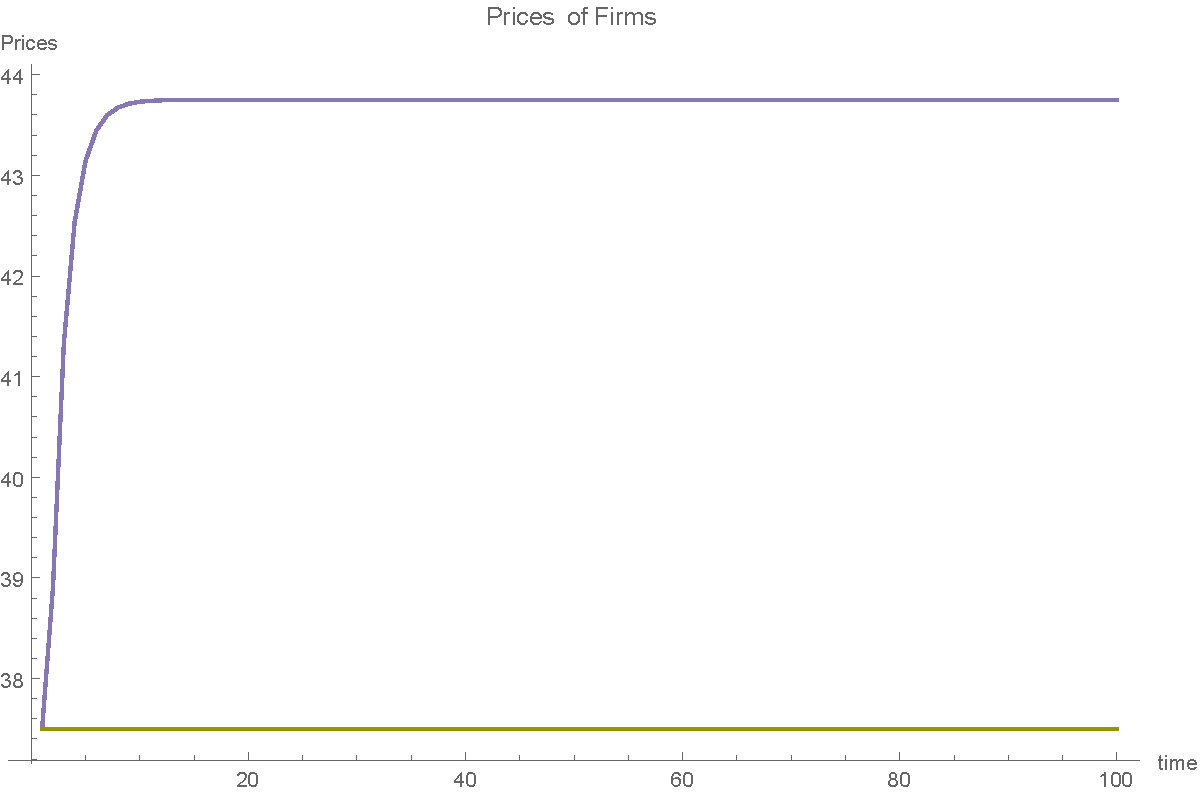
\includegraphics[scale=0.35]{../Plots/prices1b}
            \caption{Preise in b)}
            \label{fig:prices1b}
       \end{figure}
    \end{column}
  \end{columns}
\end{frame}

\begin{frame}{Preise (c)}
\begin{columns}[T]
    \begin{column}{.3\textwidth}
      \begin{itemize}
      \item Die Preise der Firmen sind identisch und konvergieren.
      \end{itemize}
      \end{column}
      \begin{column}{.7\textwidth}
      \begin{figure}[t]
            \centering
            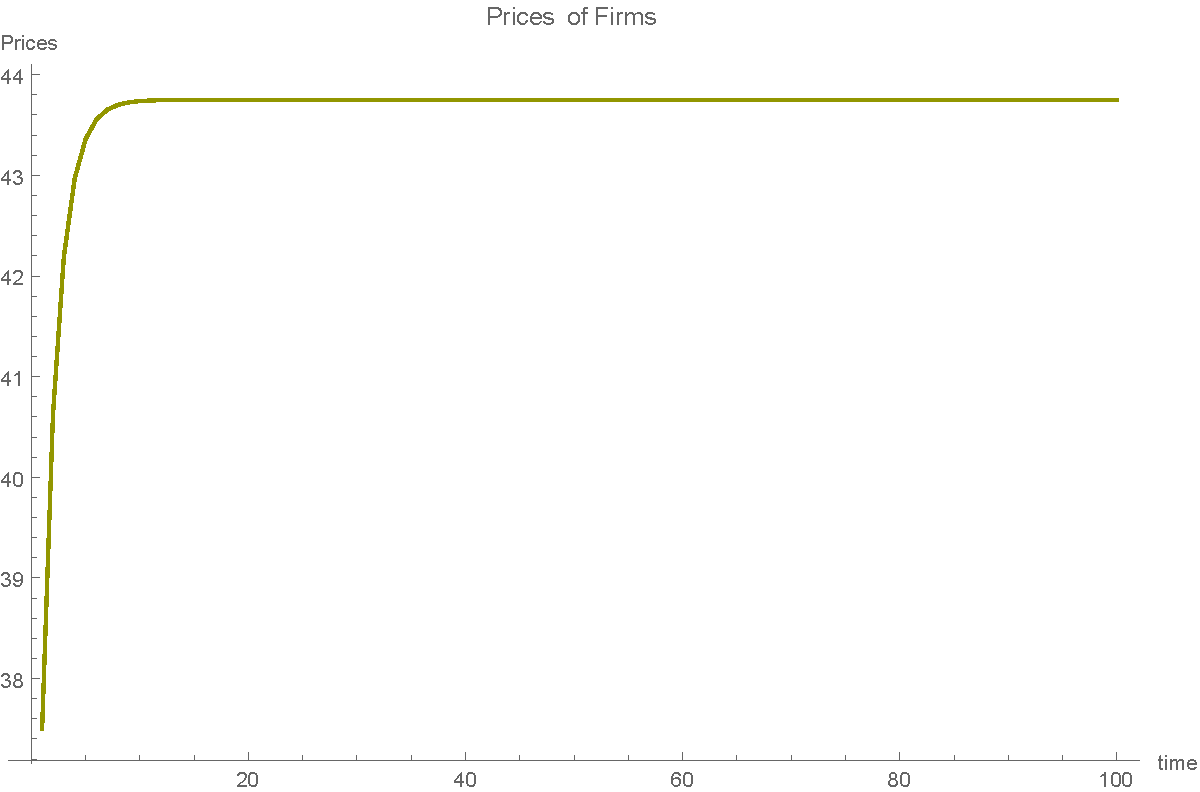
\includegraphics[scale=0.35]{../Plots/prices1c}
            \caption{Preise in c)}
            \label{fig:prices1c}
       \end{figure}
    \end{column}
  \end{columns}
\end{frame}

\section*{}
\begin{frame}
\centering
 Vielen Dank für die Aufmerksamkeit!
\end{frame}

\end{document}